% Time-Stamp: <2020-08-12 13:07:42 misho>


\documentclass[CheatSheet]{subfiles}
\newcommand{\ddP}[2][3]{\frac{\dd^{#1}\vc#2}{(2\pi)^{#1}}}

\begin{document}
\summarystyle
\section{Cosmology}
\paragraph{FLRW metric} With a scale factor normalized by $a(t_0)=1$,\\
\begin{minipage}{0.6\textwidth}
\begin{equation}
  \dd s^2 = \dd t^2-a^2(t)\left[
  \frac{\dd r^2}{1-K r^2}+r^2\dd\theta^2+r^2\sin^2\theta\dd\phi^2
\right]
\end{equation}\vspace{-2em}
\begin{align*}
\text{comoving coordinate~~}& \vc r=(r\sin\theta\cos\phi,r\sin\theta\cos\phi,r\cos\theta),\\
\text{proper coordinate~~}& \vc x(t)=a(t)\vc r,\\
\text{comoving distance~~}& \chi_{AB}=\int_{r_A}^{r_B}\frac{\dd r}{\sqrt{1-Kr^2}},\\
\text{proper distance~~}& d_{AB}(t)=a(t)\chi_{AB}.
\end{align*}
\end{minipage}
\begin{minipage}{0.395\textwidth}
\hfill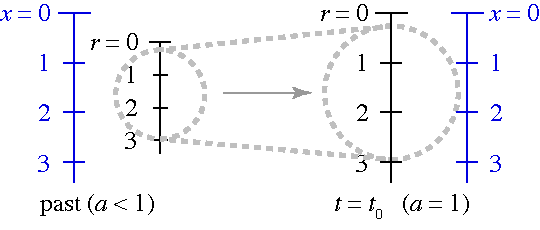
\includegraphics[width=0.9\textwidth]{figs/expansion.pdf}
\end{minipage}

\vspace{0.5em}

Ricci tensor and scalar are given by
\begin{alignat}{3}
 &R_{00}=\tensor{R}{^0_0}=\frac{3\ddot a}{a}, \qquad&
 &R_{0i}=R_{i0}=\tensor{R}{^0_i} = \tensor{R}{^i_0}=0, \qquad&
 &R_{ij}\neq 0,\notag
\\
 &\tensor{R}{^i_j} = \delta^i_j\left(\frac{\ddot a}{a} + \frac{2\dot a^2}{a^2} + \frac{2K}{a^2}\right);\qquad&
 &R = 6\left(\frac{\ddot a}{a} + \frac{\dot a^2}{a^2} + \frac{K}{a^2}\right).
\end{alignat}


\paragraph{Particle density}For a massless particle, with $L^\pm_n=\pm\mathop{\text{\texttt{PolyLog}}}(n,\pm\ee^{\mu/T})$ and arrows denoting $\mu\to0$,
\begin{alignat}{4}
 n\w{MB}    &=\frac{\ee^{\mu/T}}{\pi^2}gT^3 &\quad&\to\frac{1}{\pi^2}gT^3,&\qquad
 \rho\w{MB} &=3Tn\w{MB}&\quad& \to \frac{3}{\pi^2}gT^4,\\
 n\w{BE}&=\frac{L^+_3}{\pi^2}gT^3 &&\to \frac{\zeta_3}{\pi^2}gT^3,&
 \rho\w{BE}&=\frac{3L^+_4}{\pi^2}gT^4&&\to\frac{\pi^2}{30}gT^4,\\
 n\w{FD}&=\frac{L^-_3}{\pi^2}gT^3&&\to\frac34\frac{\zeta_3}{\pi^2}gT^3,&
 \rho\w{FD}&=\frac{3L^-_4}{\pi^2}gT^4&&\to\frac78\frac{\pi^2}{30}gT^4,
\end{alignat}

For massive particle, with $x=m/T$ and $K_n(x)=\mathop{\text{\texttt{BesselK}}}(n,x)$,
\begin{alignat}{3}
 n\w{MB}&=g\ee^{\mu/T}\cdot\frac{T^3}{2\pi^2}x^2K_2(x)\qquad
&\stackrel{x\gg1}\longrightarrow&~
g\ee^{\mu/T}\frac{T^3}{(2\pi)^{3/2}}x^{3/2}\ee^{-x},\\
\rho\w{MB}&=\left(3+\frac{xK_1(x)}{K_2(x)}\right)Tn\w{MB}
&\stackrel{x\gg1}\longrightarrow&~
\left(m+\frac{3}{2}T+\frac{15T^2}{8m}\right)n\w{MB},\qquad&
 p\w{MB}&=T n\w{MB}.
\end{alignat}


\detailstyle

\clearpage

\subsection{FLRW metric}
Two conventions are known for FLRW \GRAY{(\russian{Фр\'{и}дман}-Lema\^{i}tre-Robertson-Walker)} metric:
\begin{align}
  \dd s^2
&= \dd t^2-a^2(t)\left[\frac{\dd r^2}{1- K r^2}+ r^2\dd\theta^2+ r^2\sin^2\theta\dd\phi^2\right]
&&\text{$[r]=\text{(length)}$, $a$ is unitless with $a(t_0)=1$}
\\
&= \dd t^2-R^2(t)\left[\frac{\dd \tilde r^2}{1-\tilde K \tilde r^2}+\tilde r^2\dd\theta^2+\tilde r^2\sin^2\theta\dd\phi^2\right]
&&\text{$[R]=\text{(length)}$, $\tilde r$ is unitless, $\tilde K=\{0,\pm1\}$}
\end{align}
related by a rescaling, $R(t)/a(t)=R(t_0)\equiv R_0$, i.e., 
$r = \tilde r R_0$ and $K = \tilde K/R_0^2$.
The curvature radius is given by $6K/a^2$ and a spherical, flat, and hyperspherical universe are respectively given by $K>0$, $K=0$, and $K<0$.

FLRW metric can have several forms. For $\{K>0,K=0,K<0\}$,
\begin{align}
\dd s^2
&= \dd t^2-a^2(t)\left(\frac{\dd r^2}{1- K r^2}+ r^2\dd\Omega\right)
&\dd\Omega &= \dd\theta^2+\sin^2\theta\dd\phi^2,
\\&= \dd t^2-a^2(t)\left[\dd\vc r^2 + \frac{K(\vc r\cdot\dd\vc r)^2}{1-K\|\vc r\|^2}\right]
&\vc r&=(r\sin\theta\cos\phi,\sin\theta\sin\phi,\cos\phi)
\\&= \dd t^2-\left[\frac{a(t)}{1 + (K/4)\rho^2}\right]^2(\dd\rho^2 + \rho^2\dd\Omega)
     &\rho&=R_0 \tilde \rho:=\frac{2r}{1+\sqrt{1-Kr^2}}=\frac{2\tilde r R_0}{1+\sqrt{1-\tilde K\tilde r^2}}
\\&= \dd t^2-\left[\frac{R(t)}{1 + (\tilde K/4){\tilde\rho}^2}\right]^2(\dd{\tilde\rho}^2 + {\tilde\rho}^2\dd\Omega)
\\
&=
\dd t^2-R^2(t)\Bigl(\dd{\tilde\chi}^2 + \{\sin\tilde\chi,\tilde\chi,\sinh\tilde\chi\}^2\dd\Omega\Bigr)
&\dd\chi&=R_0\dd\tilde\chi = \frac{\dd r'}{\sqrt{1-K r'^2}}
\quad\text{[comoving distance]}
\\
&=a^2(t)\Bigl(
\dd\eta^2-\dd{\chi}^2 - R_0^2\{\sin\tilde\chi,\tilde\chi,\sinh\tilde\chi\}^2\dd\Omega
\Bigr)
&\dd\eta& := \frac{\dd t'}{a(t')}
\quad\text{[conformal time]}.
\end{align}
Explicitly, $\chi$ is given by
\begin{equation}
 \chi
  = \int_0^r\frac{\dd r'}{\sqrt{1-K r'^2}}
  = \int_0^{\tilde r}\frac{R_0\dd \tilde r'}{\sqrt{1-\tilde K \tilde r'^2}}
  = R_0\{\sin^{-1}\tilde r,\tilde r,\sinh^{-1}\tilde r\}
  = 2R_0\left\{\tan^{-1}\frac{\tilde \rho}{2}, \frac{\tilde\rho}{2},\tanh^{-1}\frac{\tilde \rho}{2}\right\}.
\end{equation}

The Christofffel symbol, Riemann tensor, Ricci tensor, and Ricci scalar are given by
\begin{align*}
 \tensor{\Gamma}{^n_i_j} &= \frac{g^{nk}}{2}(g_{jk,i}+g_{ik,j}-g_{ij,k}),
 &\tensor{R}{_i_j_k^l} &=
 \tensor{\Gamma}{^l_{jk,i}}
 -\tensor{\Gamma}{^l_{ik,j}}
 +\tensor{\Gamma}{^a_j_k}\tensor\Gamma{^l_a_i}
 -\tensor{\Gamma}{^a_i_k}\tensor\Gamma{^l_a_j}\footnotemark,
& {R}_{ij}&=\tensor{R}{_i_k_j^k},
& R &= g^{ij}R_{ij}.
\end{align*}
\footnotetext{Overall sign is convention-dependent.}



\subsection{Particle cosmology}
The particle number density, pressure, and energy density are calculated from distribution functions:
\begin{alignat}{3}
 f\w{MB}(\vc k)&=\frac{g}{\ee^{(E-\mu)/T}},\qquad&
 f\w{BE}(\vc k)&=\frac{g}{\ee^{(E-\mu)/T}-1},\qquad&
 f\w{FD}(\vc k)&=\frac{g}{\ee^{(E-\mu)/T}+1};
\end{alignat}
\begin{alignat}{3}
 n   &=\int\ddP{k}f(\vc k),\qquad&
 \rho&=\int\ddP{k}Ef(\vc k),\qquad&
 p   &=\int\ddP{k}k_zv_z f(\vc k)
      =\int\ddP{k}\frac{k^2\cos^2\theta}{E} f(\vc k).
\end{alignat}
Note the pressure is (momentum)$\times$(flux per time) on a ``wall''; assuming MB, $p=\rho/3$ for $m\ll T$ and $p=T\rho/m$ for $m\gg T$.

A thermal average of a cross section $\sigma(s)$ is schematically given by
\begin{equation}
 \vev{\sigma v}_{AB\to12\cdots n}(T)
=\frac{1}{n_An_B}\int\ddP{k_A}\ddP{k_B}\left(
f_A f_B\right)\Bigl\{\phi_1 \cdots \phi_n\sigma(s)\Bigr\}
v_{\text{M\o l}};\qquad \phi_X = \ee^{(E-\mu)/T}f_X/g,
\end{equation}
Here, the final state statistical factor $\phi_1\cdots\phi_n$ are subject to the phase space integral of the calculation of $\sigma(s)$. They are specifically given by $\phi\w{MB}=1$, $\phi\w{BE}=1+f\w{BE}/g$, and $\phi\w{FD}=1-f\w{FD}/g$.
Similarly, a thermal averaged decay rate is given by
\begin{equation}
 \vev{\Gamma}_{A\to12\cdots n}
=\frac{1}{n_A}\int\ddP{k_A}
f_A \left\{\phi_1 \cdots \phi_n
\frac{m_A}{E_A}\Gamma\right\}.
\end{equation}


With MB approximation,
\begin{align}
 \vev{\sigma v}
&=
\frac{g_Ag_B}{n_An_B}
\ee^{(\mu_A+\mu_B)/T}
\int\ddP{k_A}\ddP{k_B}
\ee^{-(E_A+E_B)/T}
\sigma(s)v_{\text{M\o l}}
\\
&=
\int\frac{\dd s\dd E_+ \dd E_-}{32m_A^2 m_B^2 T^2 K_2(m_A/T)K_2(m_B/T)}
\ee^{-E_+/T}
4E_AE_B\sigma(s)v_{\text{M\o l}}\quad(\text{$\times1/2$ if $A=B$)}
\\
&=
\frac{1}{16m_A^2 m_B^2 T K_2(m_A/T)K_2(m_B/T)}
\int
\frac{K_1(\sqrt{s}/T) \dd s}{\sqrt{s}}
\sqrt{\Kallen(s,m_A^2,m_B^2)}
\cdot2E_A2E_Bv_{\text{M\o l}}\sigma(s)
\quad(\times1/2),
\\
 \vev{\Gamma}
 &=\frac{K_1(m_A/T)}{K_2(m_A/T)}\Gamma.
\end{align}

\end{document}
